\documentclass[a4paper,10pt]{article}

%\usepackage[utf8]{inputenc}
\usepackage{graphicx}
\usepackage{url}
\usepackage{float}
\usepackage{times}
\usepackage{multirow}
\usepackage{listings}
\usepackage{times}
\usepackage{paralist}
\usepackage{epsfig}
\usepackage{subfigure}
%\usepackage[hypertex]{hyperref}
\usepackage[pdftex]{hyperref}
\usepackage{subfigure}
\usepackage{color}
\usepackage{ifpdf}
\usepackage{wrapfig}

\usepackage{texdraw}
\usepackage{epsf}
\usepackage{array}
\usepackage{cite}
\usepackage{enumitem}
\usepackage{verbatim}
\usepackage{setspace}
\sloppy
\usepackage{geometry}



\newcommand{\I}[1]{\textit{#1}}
\newcommand{\B}[1]{\textbf{#1}}
\newcommand{\BI}[1]{\textbf{\textit{#1}}}
\newcommand{\T}[1]{\texttt{#1}}
\newcommand{\dctf}{dC$_{25}$ }
\newcommand{\dctfnsp}{dC$_{25}$}
\newcommand{\atf}{A$_{25}$ }
\newcommand{\dco}{dC$_{1}$ }
\newcommand{\atfnsp}{A$_{25}$}
\newcommand{\dconsp}{dC$_{1}$}
\newcommand{\aonsp}{A$_{1}$}
\newcommand{\ao}{A$_{1}$ }
\newcommand{\ato}{A$_{1}$ }
\newcommand{\ahl}{$\alpha$HL }
\newcommand{\ahlnsp}{$\alpha$HL}
\newcommand{\prim}{$^{\prime}$ }
\newcommand{\primnsp}{$^{\prime}$}


\pdfpagewidth 8.5in
\pdfpageheight 11in 

\setlength\topmargin{0in}
\setlength\headheight{0in}
\setlength\headsep{0in}
\setlength\textheight{9in}
\setlength\textwidth{6.5in}
\setlength\oddsidemargin{0in}
\setlength\evensidemargin{0in}
\setlength\parindent{0.1in}
\setlength\parskip{0.25em}

\ifpdf
 \DeclareGraphicsExtensions{.pdf, .jpg, .png}
\else
 \DeclareGraphicsExtensions{.eps, .ps}
\fi

\newcommand{\up}{\vspace*{-1em}}
\newcommand{\upp}{\vspace*{-0.5em}}
\newcommand{\tc}{$T_c$ }
\newcommand{\ttc} {TTC}
\newcommand{\tcc}{TCC}

\newcommand{\jha}[1]{ {\textcolor{red} { ***Jha: #1 }}}

\begin{document}
\title{\Large Request for Supplemental Allocation}

\author{Principal Investigator: Shantenu Jha$^{1,2}$ \\ Co-Principal Investigator: Joohyun Kim$^{1}$ \\ Co-Principal Investigator: Yaakoub El Khamra$^{3}$\\\
   \small{\emph{$^{1}$Center for Computation \& Technology, Louisiana State University, Baton Rouge,
USA}}
\\
  \small{\emph{$^{2}$Rutgers, State Univeristy of New Jersey, USA}}
\\
  \small{\emph{$^{3}$Texas Advanced Computing Center TACC, University of Texas, Austin, USA}}}

\newif\ifdraft
\drafttrue
\ifdraft
\newcommand{\amnote}[1]{ {\textcolor{magenta} { ***AM: #1c }}}
\newcommand{\jhanote}[1]{ {\textcolor{red} { ***SJ: #1 }}}
\newcommand{\yyenote}[1]{ {\textcolor{blue} { ***YYE: #1 }}}
\newcommand{\michaelnote}[1]{ {\textcolor{blue} { ***MM: #1 }}}
\else
\newcommand{\amnote}[1]{}
\newcommand{\jhanote}[1]{}
\newcommand{\yyenote}[1]{}
\newcommand{\michaelnote}[1]{ {\textcolor{blue} { ***MM: #1 }}}
\fi


\date{01 April 2011}

\maketitle

\section{Summary}

We would  like to request a supplemental allocation on TeraGrid resources. In the first year of our multi--year allocation (TG-MCB090174: {\it Scale-Up and Scale-Out of Ensemble-based Simulations}) we requested 5 million SUs on Ranger and 3 million SUs on Kraken. Our allocation was awarded half the requested SUs on Ranger (2.5 million) and 2 out of 3 million SUs on Kraken.

As we have pursued our science unhindered, we have run-out of SUs half-way through the year. We have over a dozen publications appearing (or soon to appear) in conferences and journals based on research conducted with our allocation, and would want to continue with our research at the same pace.

We document progress made along multiple fronts in the short period of time in the attached progress report.  As it stands, our research will stall in the third week of April and remain that way for several months. We request 1.5 million SUs on Kraken and 1 million SUs on Ranger to tide us over to the next allocation renewal cycle, when we will be eligible to request an advance on our second--year allocation. This will allow us to continue our work and productivity for the next few months.

\section{The Case for Continuity}

As outlined in the progress report, we have delivered impressive scientific and technological advances in the short period since this grant was awarded. This includes over a dozen publications appearing in journals/conferences or in preparation. Importantly, we are on the trajectory that we were aiming for and are set to deliver on the goals that we hoped the allocation would facilitate.  Specifically, the uninterrupted continuation is important as, (i) Project 2 forms the basis for {\it specialized} runs on the DE Shaw Anton machine, to which we will have access starting in Q2 of 2011, (ii) Projects 3 is an important component of the International Interoperability Project (between TeraGrid and DEISA), (iii) Project 5 will lead to the timely delivery of an infrastructure that in turn will be used by multiple biomolecular simulation groups on the TeraGrid for efficient and effective execution of ensemble-based simulations.
%It is our hope that our scientific progress and trajectory will not be perturbed;
We would like to maintain the pace of the progress we are making; additionally, it is important to mention that several graduate dissertations and papers critically depend upon non-disruption. In the next 3-6 months, we anticipate 3 Graduate student led publications and 2 theses (1 PhD (Wei Huang) and 1 Masters (Abhinav Thota)) based upon a continued allocation.

\begin{table}
\caption{Status of subprojects and estimated requirements}
\label{table:tab1}
\begin{tabular}{ |  p{5cm} | l | l | l |}
\hline
Type of Calculation & Method or Package & HPC Resources To Be Used & SUs required\\ \hline \hline
Atomistic MD Simulation MM-PBSA & NAMD AMBER & Ranger & 1000K\\ \hline
AEE/EGFRs (50K atoms) & Amber & Kraken & 1500K\\ \hline
Total SUs  &   & Ranger/Kraken & 2500K \\ \hline
\end{tabular}

\end{table}

Table~\ref{table:tab1} shows the current status of the main stages of the projects in the allocation and the estimated computational requirements. The resource justification is as follows:

\jhanote{This section and the next one require attention, better justification. Sorry I just took the more demanding aspects of the proposal and placed them as yet to be finished simulations}

\subsection{Project 2 Resource Justification}

Riboswitches are regulatory RNAs that control the expression of downstream genes. Small metabolite molecules, such as amino acids, nucleotides, coenzymes etc., can bind to riboswitches as effectors in vivo~\cite{mandal}.  In our recent research efforts, the SAM-I riboswitch, one member of the riboswitch family that regulates genes related to the metabolism of sulfur and methionine, has been extensively investigated with atomistic simulations.  This riboswitch choose alternative conformation depending on binding of a S-adenosyl methionine (SAM).  When a SAM is bound, the aptamer domain forms anti-anti-terminator (AAT) conformation, which turns off the downstream genes by forming the terminator (T). Otherwise, the anti-terminator (AT) is formed prohibiting the T element formation for continuing transcription process (see Fig.~\ref{fig:ribo-pipeline}(b)~\cite{brooke}).  Although the structures of the SAM-I riboswitch in the anti-anti-terminator (AAT) conformation have been solved via X-ray crystallography, it is just a static view of how SAM binds to the SAM-I riboswitch RNA.

\begin{figure}
\begin{center}
  \subfigure[]{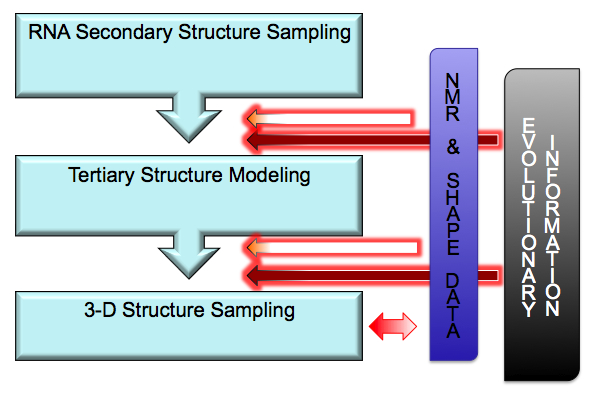
\includegraphics[scale=0.33]{flowchart-pipeline}}
  \subfigure[]{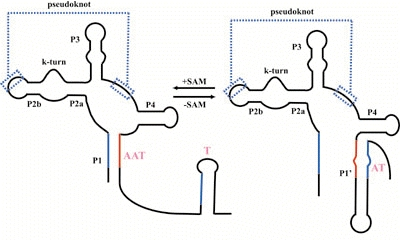
\includegraphics[scale=0.55]{ss-schema}}
\end{center}
\up\up
\caption{(a) The pipeline for riboswitch structure prediction and binding affinity estimation (b) Schematic of the secondary structure change displayed by the SAM-I riboswitch (The left figure represents the OFF state resulted by the SAM-binding and the right figure represents the ON state)}
\label{fig:ribo-pipeline}
\up
\end{figure}

Our current research goals can be understood readily using the pipeline illustrated in Fig.~\ref{fig:ribo-pipeline} and the required computational tasks carried out with the allocation of this request are described below. With the proposed pipeline, we aim to investigate folding dynamics of ribsowtich RNAs and closely related RNA-ligand binding affinity.  This is in contrast to our earlier strategy during which we have heavily relied only upon all-atom Molecular Dynamics simulations.  Indeed, combining multiple computational approaches that differ in their physical principles, increase the chance to achieve a comprehensive understanding of the complex biological process carried out by riboswitch RNAs.  The entire pipeline comprises three steps; the first step represents the Boltzmann Ensemble (BE) sampling of RNA secondary structures, the second step is about the 3D modeling from 2D structure information, and the third step carries out the conformational sampling.  Note that sampling in the first step is executed using RNA secondary structure prediction algorithms, employing the nearest-neighbor energy model and thermodynamics parameters that are experimentally estimated.  The third step is carried out with all-atom MD simulations. The second step represents 3-D molecular modeling using 2-D information.  The requested allocation is primarily support the computational requirements corresponding to the first and the third stages. The BE sampling for the first step is conducted with SFold package\cite{ding2006}.  This type of sampling is typically carried out without the abilitiy to concurrently run multiple simulations, but recently, thanks to the development of a novel runtime environment, we have demonstrated the ``parallel sampling'' of RNA secondary structures using scalable HPC resources (See "Emerging Computational Methodologies in Life Science"~\cite{ecmls10}). For all-atom MD simulations, protocols similar to previous years will be used as described below. As a matter of fact, our pipeline represents the energy landscape perspective that interprets the folding dynamics of a RNA with statistical treatment of an ensemble of structures distributed in the pertinent energy landscape~\cite{onuchic1997}, which has been successfully applied for protein folding but not fully applied for RNA folding\cite{cupal1997}. In our pipeline, the entire folding configuration space is efficiently explored by RNA secondary structure sampling and successively atomistic MD simulations explore the relevant basins of attraction starting from the configurations sampled.

While our pipeline can serve as a de-novo tool for RNA structure prediction from a sequence, it can also be used as a tool box that is able to carry out different physics-based calculations corresponding to each layer, i.e., RNA secondary structure prediction, 3D modeling, and all atom MD simulations for different scientific aims.  This is related to the fact that the nature of RNA folding occurs in a hierarchical manner, implying that the first and the third steps can deal with its own biophysical problems but later findings can be combined for an integrated perspective. Furthermore, our framework uses various computational approaches whose performance relies upon the availability of effective parallel implementation, thus benefiting from TeraGrid like federated, distributed and massively parallel resources.

\begin{figure}
\begin{center}
  \subfigure[]{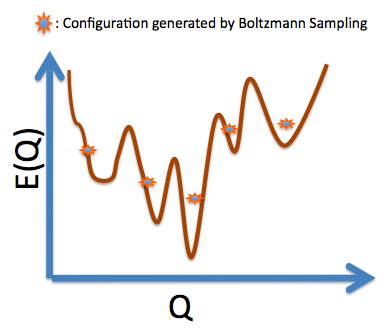
\includegraphics[scale=0.33]{el}}
  \subfigure[]{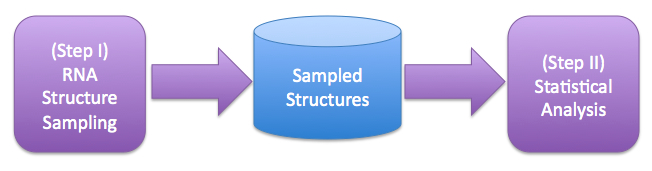
\includegraphics[scale=0.4]{pipeline}}
\end{center}
\up\up
\caption{(a) Illustration of structure sampling in configuration space.  (b) Schematic of a workflow for sampling and analysis of RNA secondary structures obtained with the Boltzmann-weighted sampling}
\label{fig:folding energy landscape}
\end{figure}

A major proportion of our allocation for this project will be used for atomistic MD simulations.  The main goal of the MD simulations is to probe the dynamic interactions between the SAM-I riboswitch and SAM at the nanoscale and to explore determinants for the specificity. In particular, we aim to examine, i) SAM-I riboswitches and their different constructs that differ from each other in potentially different secondary structures and tertiary interactions, ii) different sequences in SAM-I family, and iii) other SAM riboswiches (SAM-II and SAM-III) for which X-ray structures were recently reported and TPP ribosiwtches that we recently started to investigate.  To estimate binding affinity, we employed the Molecular Mechanics - Poisson Boltzmann Surface Area (MM-PBSA) approach using configuration from MD simulations.  As for efficient sampling of conformational dynamics, replica exchange molecular dynamics (REMD) protocol will be used.  REMD calculations will be carried out using available scripts or with our recent development for the distributed adaptive REMD.  

The protocols to be employed are similar to previous protocols.  We will start with a structure derived from the X-ray crystal structures of the AAT conformation of SAM-I riboswitch (PDB: 2GIS, 3GX2, 3GX3, 3GX5, 3GX6, 3GX7)~\cite{montange} or configurations generated by a process via two layers of the pipeline. For a free state riboswitch, SAM is directly removed from the x-ray crystal structure and replaced with solvent water. The amber99bsc0 correction force field is used here~\cite{alberto}. Parameters for SAM are from the Generalized Amber Force Field (GAFF) and missing parameters are calculated using ANTECHAMBER~\cite{wang}. Positions of added hydrogens are guessed using PSFGEN within NAMD 2.6. Then the RNA molecules are solvated in a cubic solvent box of TIP3P waters with a 1.6 nm padding in all directions. Sodium and magnesium ions are distributed around the RNA molecules and neutralize charge of the system. The total number of atoms in the system is 56,000. Energy minimizations are carried out to remove bad contacts. Starting from 0 K, the temperature is raised 10 K every 10,000 steps, and is held constant after reaching the desired temperature (310 K) using temperature reassignment. MD simulations are performed in the NPT ensemble with the pressure maintained using the Langevin piston method with a period of 100 fs and decay times of 50 fs. The time step is 2fs for both equilibration and production phase. Bond lengths between hydrogens and heavy atoms are constrained using SHAKE. The long-range electrostatics is treated with the Particle Mesh Ewald (PME) method with a cutoff distance 1.2 nm.  We use NAMD 2.6.


\begin{figure}%{r}{0.4\textwidth}
\begin{center}
  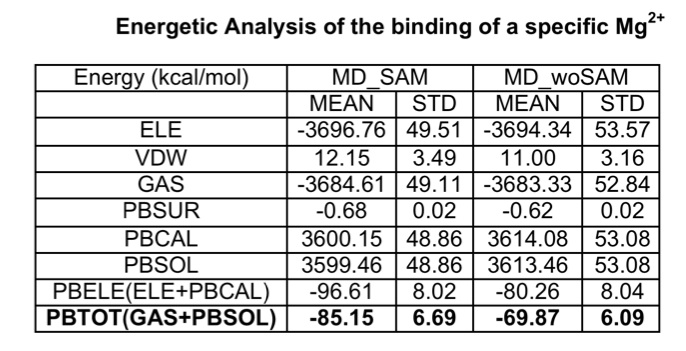
\includegraphics[scale=0.4]{mm-pbsa-mg}
   \caption{MM-PBSA estimation on ${Mg^{2+}}$ binding with a SAM-I riboswitch RNA}
\up\up
\label{fig:mm-pbsa-mg-table}
\end{center}
\end{figure}

Obtained trajectories will be analyzed with various statistical techniques.  Generally, beyond straightforward trajectory analysis measuring various structural variables, PCA analysis and clustering are useful to extract characteristic dynamical motions in terms of reduced dimension techniques\cite{kimjpcb2010, SAM-I-NAR2009}.   Also, we consider the calculations utilizing the Inherent Structure formalism that might reveal intriguing information with respect to the energy landscape properties such as basins, minima, and saddles\cite{kimpre2002,kimjcp2004}.  Conformational dynamics from obtained trajectories of a complex with a ligand and free state will be used for the MM-PBSA calculation with which ligand binding affinity of the metabolites, SAM, or TPP or other related ligands and also for cation binding of ${Mg^{2+}}$ is estimated.  In particular, ${Mg^{2+}}$ binding has been evidenced as crucial for function of catalytic RNAs but remains as elusive for detailed roles in folding dynamics of riboswitches.  Our preliminary results for cation binding are presented in Fig~\ref{fig:mm-pbsa-mg-table}.  According to our preliminary results, this protocol is useful for ranking ligands that bind a pertinent riboswitch, but also we observed that the accuracy depends on the way for entropy calculation and the use of configurations from MD trajectories.  Also, more challenging questions relevant to the validity of force fields that ignores the polarizability as well as the charge transfer effect should be investigated and we hope our calculations provide interesting clues for the answer.      

Sampling the Boltzmann ensemble of RNA secondary structures is the primary strategy to explore the energy landscape efficiently.  We use the SFold pacakge\cite{ding2006} for sampling. The sampling of structures with an input sequence of riboswitches is not computationally intensive, but a considerable number of tasks are required depending on the biological questions.  For example, we carry out comparative investigation on all riboswitches of the same family identified in RFam database; at the moment 2092 SAM-I riboswitches are identified, and the number grows as more genomes are added.  Also, after a sampling step, the analyses involve multi-stage heterogeneous tasks (see Fig.~\ref{fig:folding energy landscape}(b)).  

We plan to simulate SAM-I aptamer RNA. Previous time-step benchmarks on Ranger indicate a computation rate of 1ns/82 hours for this 56K atom system on 32 cores.

According to our recent benchmarks on Ranger, when using 32 cores, the time taken per MD step is approximately 0.06s for a SAM-I aptamer RNA; thus the wall clock time required to complete 1ns is 0.34 day; in other words for a 56K system, 1 ns simulations require $\approx$ 300 CPU hours.  Thus each 100 ns simulation requires approximately 30,000 CPU hrs.  Analysis~\cite{SAM-I-NAR2009} results indicate that more than 300 ns trajectory is desirable for observing meaningful conformational dynamics. Therefore, without additional post-analysis including MM-PBSA calculations, a rough estimation suggest that we can obtain about 100 simulations of a similar system with 900,000 SUs (See {\url{http://staging.teragrid.org/userinfo/aus/namd_benchmark.php}} Boltzmann Ensemble sampling. The total requested to finish this project is 1 million SUs on Ranger.

\subsection{Project 3 Resource Justification}
The epidermal growth factor receptor (EGFR) is an especially important enzyme target in lung cancer therapy because it mutates and/or is overexpressed in most non-small cell lung carcinoma (NSCLC) tumours. Inhibition of kinase activation of EGFR is a frequently used method to suppress its functions \cite{bib:nature_tki}. The majority of tyrosine kinase inhibitors (TKIs) are ATP-competitive inhibitors which bind in the ATP-binding site. Molecular dynamics (MD) simulations will be used to study the structural and energetic properties of inhibitor-EGFR complexes. The binding affinity of inhibitors to EGFRs will be calculated by molecular mechanics Poisson-Boltzmann surface area (MM/PBSA) methods \cite{bib:wan_philtrans}. This molecular level study is one component of the EU FP7 ContraCancrum (Clinically Oriented Translational Cancer Multilevel Modeling) project which aims at developing a composite multilevel platform for simulating malignant tumor development and pharmacologic responses to a therapeutic intervention (http://www.contracancrum.eu). We have employed large scale MD techniques using both TeraGrid and DEISA resources in order to study the interactions of inhibitors with wild-type and mutant EGFRs \cite{bib:wc2009}.

A better understanding of the reasons for the success or failure of a therapeutic intervention will help us in the selection of subgroups of patients who are most likely to respond to specific drugs, and paves the way for personalized treatment \cite{bib:hiv}. We have already performed a preliminary study of different inhibitors (AEE788, AFN941 and gefitinib) with EGFR which we now intend to extend to look at a wider variety of inhibitors and EGFR mutations and to probe longer time scale motions of the protein. Planned simulations include ensembles of 50, 50,000 atoms with 25 runs each. Each simulation lasts for 4ns and runs for 9 hours on 128 cores. We therefore request 1.5 million SUs on Kraken to finish this project. The ensemble size and number of runs are typical of established studies~\cite{bib:wan_philtrans,bib:wc2009}.

\subsection{Other projects}
In conjunction with the scientific questions we are addressing, we are also involved in the development of a runtime execution system (DARE) that uses the Simple API for Grid Applications (SAGA: http://saga.cct.lsu.edu/) and SAGA-based Pilot-Job (BigJob) to allow the running and coordination of hundred if not thousands of large-scale ensembles across resources, both on the TeraGrid and the EU DEISA network, as part of the NSF-HPCOPS funded Interoperability Project. Significant progress has recently been achieved in allowing the use of SAGA to interoperate between these two different grids.  A key goal of an extended allocation would be to further develop this infrastructure and assess performance using real scientific workloads, and make it available for the broader \& larger community of biomolecular simulators.


%\jhanote{Yaakoub, what other sob story should we sell?}
%\yyenote{Well that pretty much covers it. Do we have a current AUS or a site project that cannot continue unless we have allocations? i.e. Matt for example. Without the SUs he's stuck doing nothing at Kraken.}

\bibliographystyle{IEEEtran}
%\bibliography{Supp,jha_loni_alloc_jul01}
\bibliography{jha_loni_alloc_jul01,ucl_trac,yye00,Supp}
\end{document}



